\documentclass{beamer}
\usepackage{ hyperref}
\usepackage[T1]{fontenc}

% other packages
\usepackage{latexsym,amsmath,xcolor,multicol,booktabs,calligra}
\usepackage{graphicx,pstricks,listings,stackengine}
\usepackage{multirow}
\usepackage{array}
\author{Chu Zhuyiheng}
\title{Something about ENKF}
% \subtitle{第一部分}
\institute{OrangeUser}
\date{2024.11.30}
\usepackage{Tsinghua}

% defs
\def\cmd#1{\texttt{\color{red}\footnotesize $\backslash$#1}}
\def\env#1{\texttt{\color{blue}\footnotesize #1}}
\definecolor{deepblue}{rgb}{0,0,0.5}
\definecolor{deepred}{rgb}{0.6,0,0}
\definecolor{deepgreen}{rgb}{0,0.5,0}
\definecolor{halfgray}{gray}{0.55}

\lstset{
    basicstyle=\ttfamily\small,
    keywordstyle=\bfseries\color{deepblue},
    emphstyle=\ttfamily\color{deepred},    % Custom highlighting style
    stringstyle=\color{deepgreen},
    numbers=left,
    numberstyle=\small\color{halfgray},
    rulesepcolor=\color{red!20!green!20!blue!20},
    frame=shadowbox,
}


\begin{document}

\begin{frame}
    \titlepage
\end{frame}

\begin{frame}
    \tableofcontents[sectionstyle=show,subsectionstyle=show/shaded/hide,subsubsectionstyle=show/shaded/hide]
\end{frame}

\begin{frame}{Key References}
    \begin{itemize}
        \item Houtekamer, P. L., \& Mitchell, H. L. (1998). \textit{Data Assimilation Using an Ensemble Kalman Filter Technique}. Monthly Weather Review, 126(3), 796–811.  
        Available at: \href{https://journals.ametsoc.org/view/journals/mwre/126/3/1520-0493_1998_126_0796_dauaek_2.0.co_2.xml}{Link to Article}

        \item Houtekamer, P. L., \& Mitchell, H. L. (2001). *A Sequential Ensemble Kalman Filter for Atmospheric Data Assimilation*. Monthly Weather Review, 129(1), 123–137.  
        Available at: \href{https://journals.ametsoc.org/view/journals/mwre/129/1/1520-0493_2001_129_0123_asekff_2.0.co_2.xml}{Link to Article}
    \end{itemize}
\end{frame}

\section{Experimental Environment}
\begin{frame}{Experimental Environment}
    Using radiosondes and satellites to observe atmospheric state, using domain averaged streamfunction error squared north of 208N at 50 kPa to measure of the error variance.
    \begin{figure}[htbp]
        \centering
            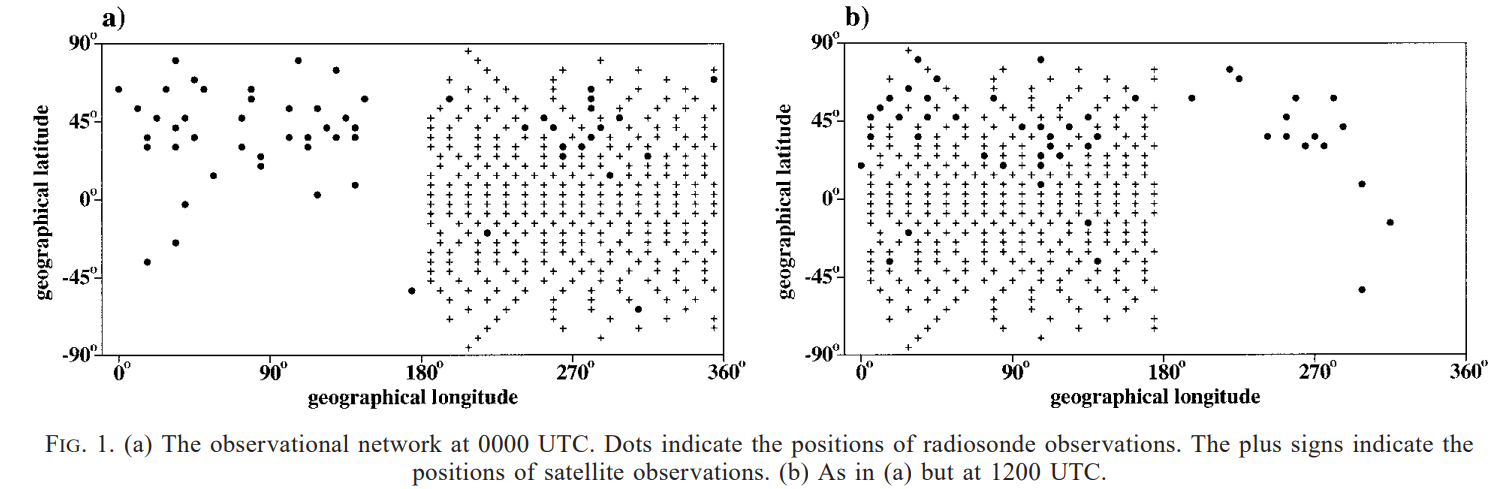
\includegraphics[width=\textwidth]{/mnt/c/workspace/study/Inverse Problem and Data Assimilation/pre/pic/env.png} % Replace with actual image file
      \end{figure}
    How to get the true state and what the stream function is are not important for understanding the subsequent ENKF part, so we will skip it.
\end{frame}

\section{Two ensembles ENKF}
\begin{frame}{Setup}
    
    \begin{figure}[htbp]
        \centering
            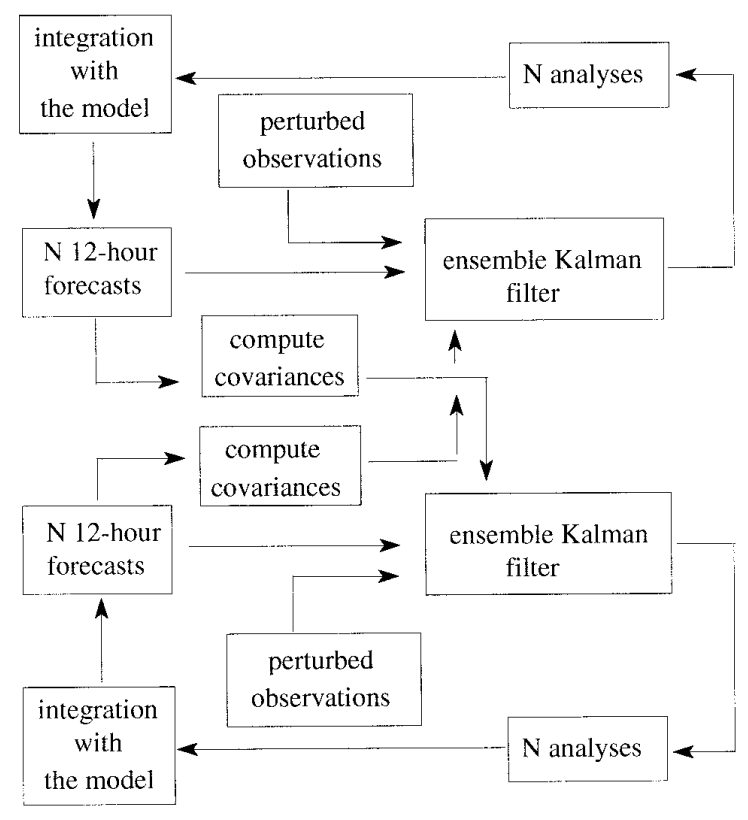
\includegraphics[width=0.5\textwidth]{/mnt/c/workspace/study/Inverse Problem and Data Assimilation/pre/pic/setup.png} % Replace with actual image file
    \end{figure}
\end{frame}
\begin{frame}{Try to use it in Project3}
    \begin{figure}[htbp]
        \centering
        \begin{minipage}[t]{0.48\textwidth}
            \centering
            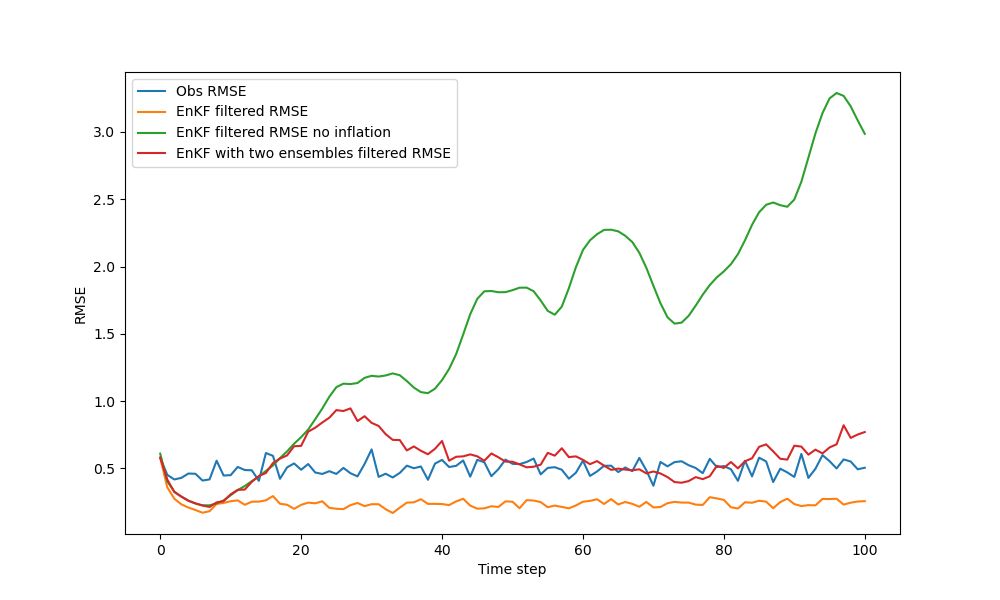
\includegraphics[width=\textwidth]{/mnt/c/workspace/study/Inverse Problem and Data Assimilation/pre/pic/ENKF_inflation.png}
        \end{minipage}
        \hfill
        \begin{minipage}[t]{0.48\textwidth}
            \centering
            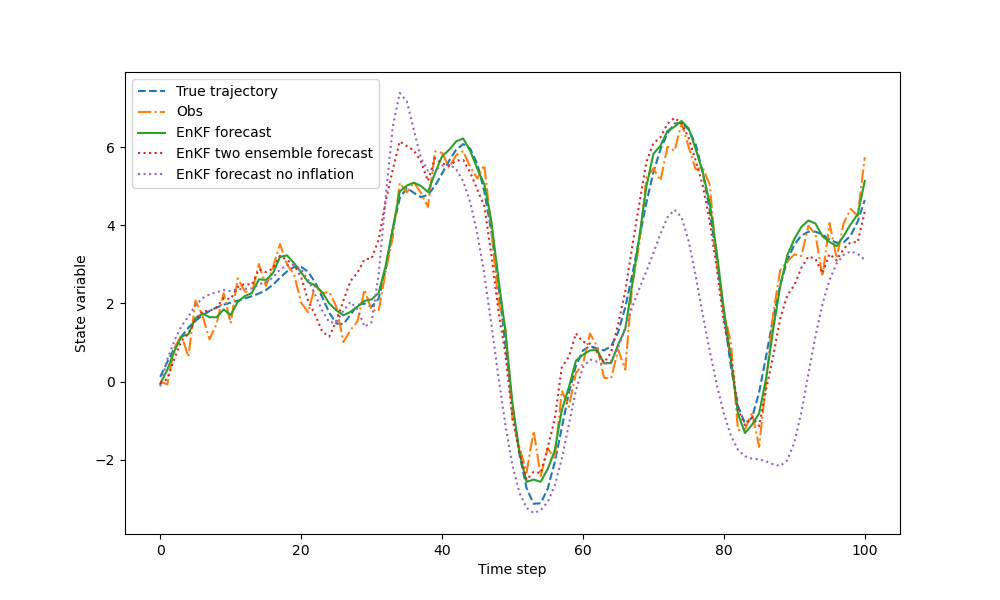
\includegraphics[width=\textwidth]{/mnt/c/workspace/study/Inverse Problem and Data Assimilation/pre/pic/ENKF_inflation_2.png} % Replace with the second image

        \end{minipage}
    \end{figure}
    The effect is not as good as using inflation, but better than not using inflation.
\end{frame}
\begin{frame}{Why it works}
    \begin{columns}[c]
        % Left column for the image
        \column{0.5\textwidth}
        \centering
        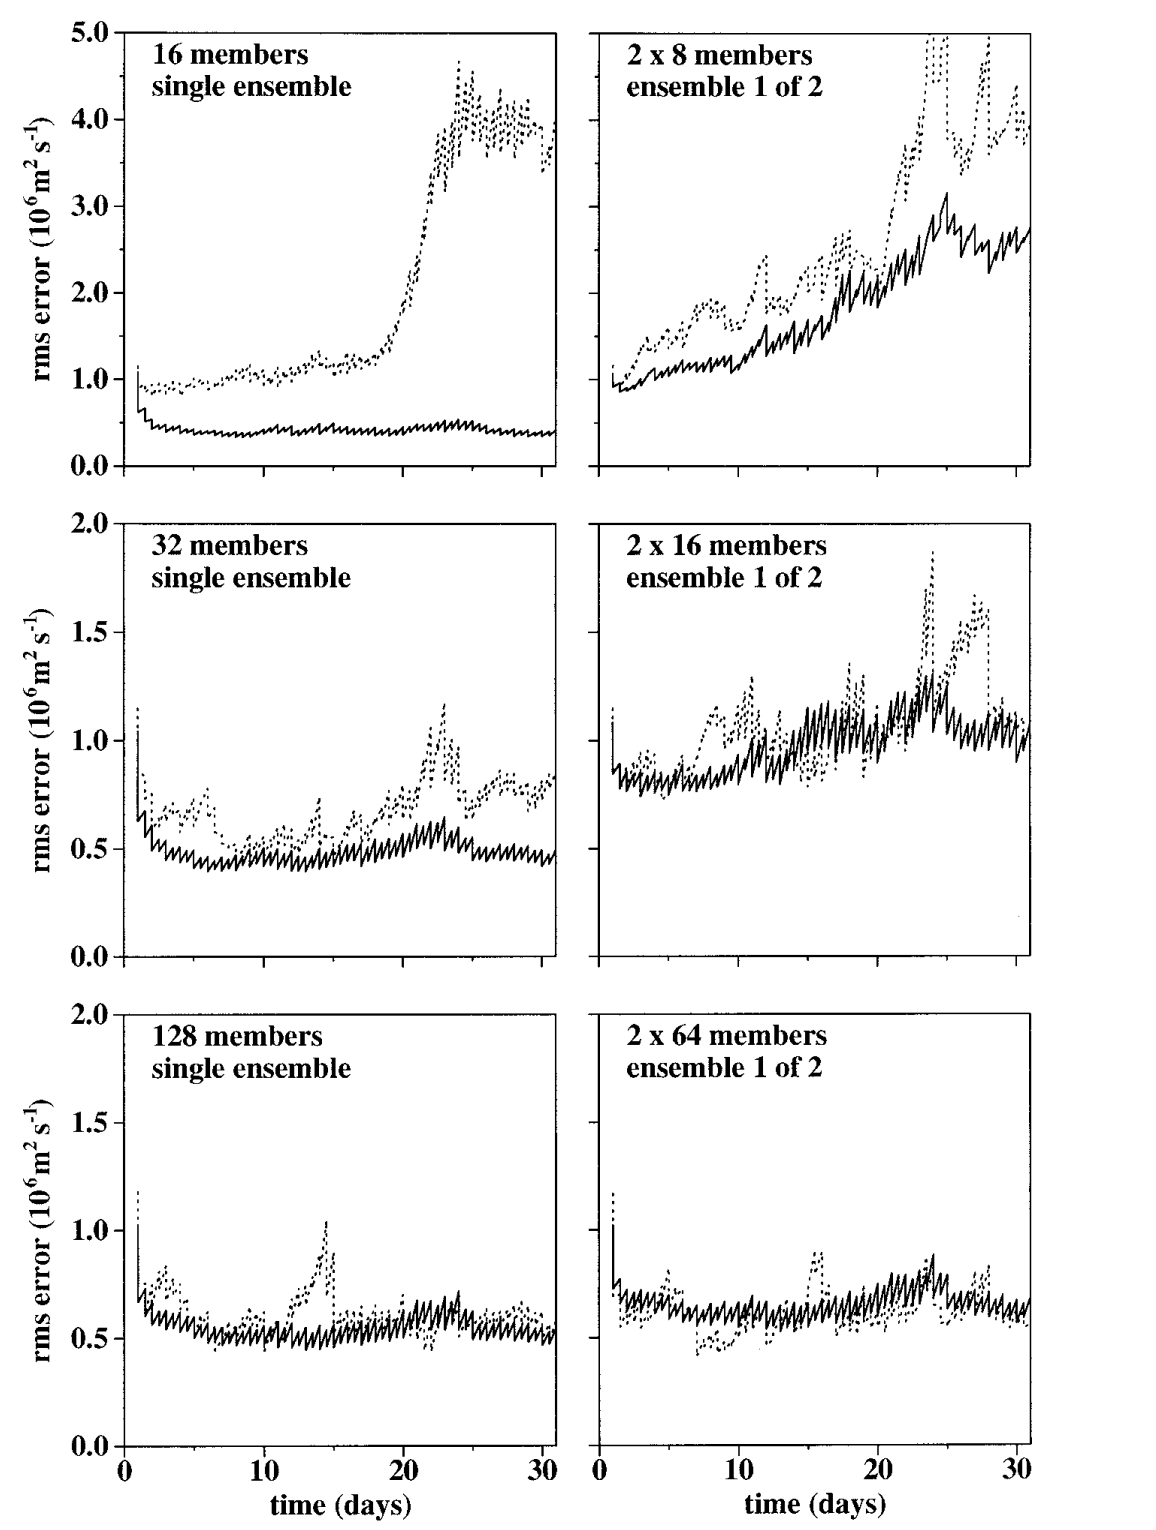
\includegraphics[width=\textwidth]{/mnt/c/workspace/study/Inverse Problem and Data Assimilation/pre/pic/rms spread and error.png} % Replace with actual image file

        % Right column for the text
        \column{0.5\textwidth}
        The solid line on the graph is the rms error, and the dotted line is the rms spread. 

        Some guesses:Perhaps when it is hard to carefully select the inflation parameter, 2 ensembles EnKF would also be a possible option?
    \end{columns}
\end{frame}

\section{Cutoff method and Schur product method}
\begin{frame}{Problem in Project2}
    I guess all students have encountered similar situations in project2?
    \begin{figure}[htbp]
        \centering
            \includegraphics[width=0.5\textwidth]{/mnt/c/workspace/study/Inverse Problem and Data Assimilation/pre/pic/killed.png} % Replace with actual image file
    \end{figure}

    This is why we need to use localization to make the matrix sparse.
\end{frame}
\begin{frame}{Cutoff method and Schur product method}
    \begin{itemize}
        \item Cutoff method:For
        each vertical column of analysis points, all the data
        within a given horizontal distance, $r_{max}$, and only that
        data, is used.
        \item Schur product method:\begin{figure}[htbp]
            \centering
                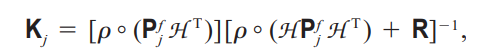
\includegraphics[width=0.5\textwidth]{/mnt/c/workspace/study/Inverse Problem and Data Assimilation/pre/pic/schur.png} % Replace with actual image file
        \end{figure}
    \end{itemize}
\end{frame}
\begin{frame}{Their results are similar}
    \begin{figure}[htbp]
        \centering
        \begin{minipage}[t]{0.48\textwidth}
            \centering
            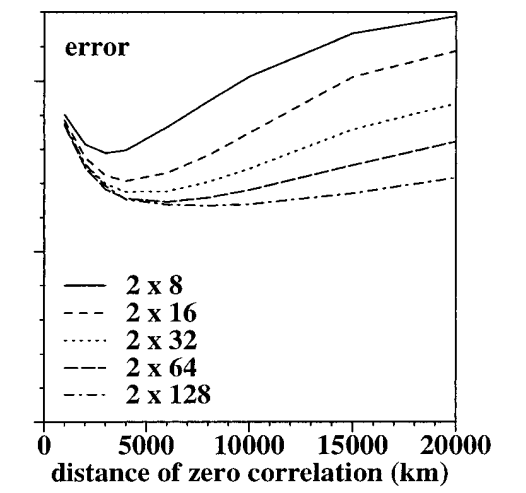
\includegraphics[width=\textwidth]{/mnt/c/workspace/study/Inverse Problem and Data Assimilation/pre/pic/schur_r.png}
        \end{minipage}
        \hfill
        \begin{minipage}[t]{0.48\textwidth}
            \centering
            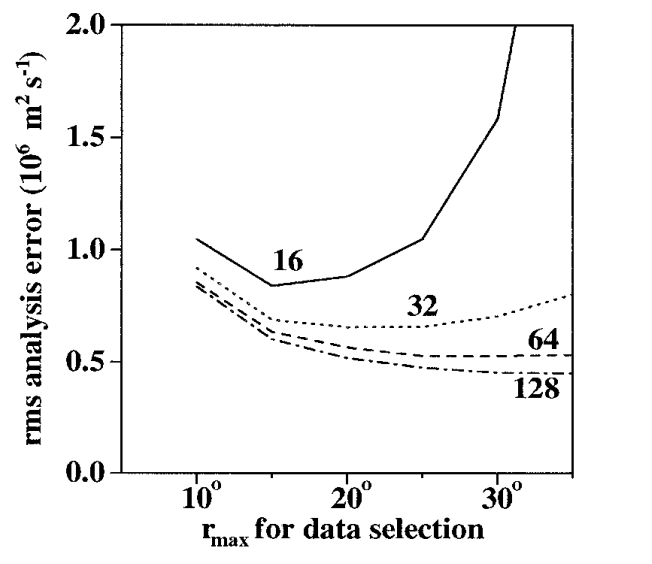
\includegraphics[width=\textwidth]{/mnt/c/workspace/study/Inverse Problem and Data Assimilation/pre/pic/cutoff_r.png} % Replace with the second image

        \end{minipage}
    \end{figure}
\end{frame}
\begin{frame}{My result}
    \begin{figure}[htbp]
    \centering
    \begin{minipage}{0.32\textwidth}
        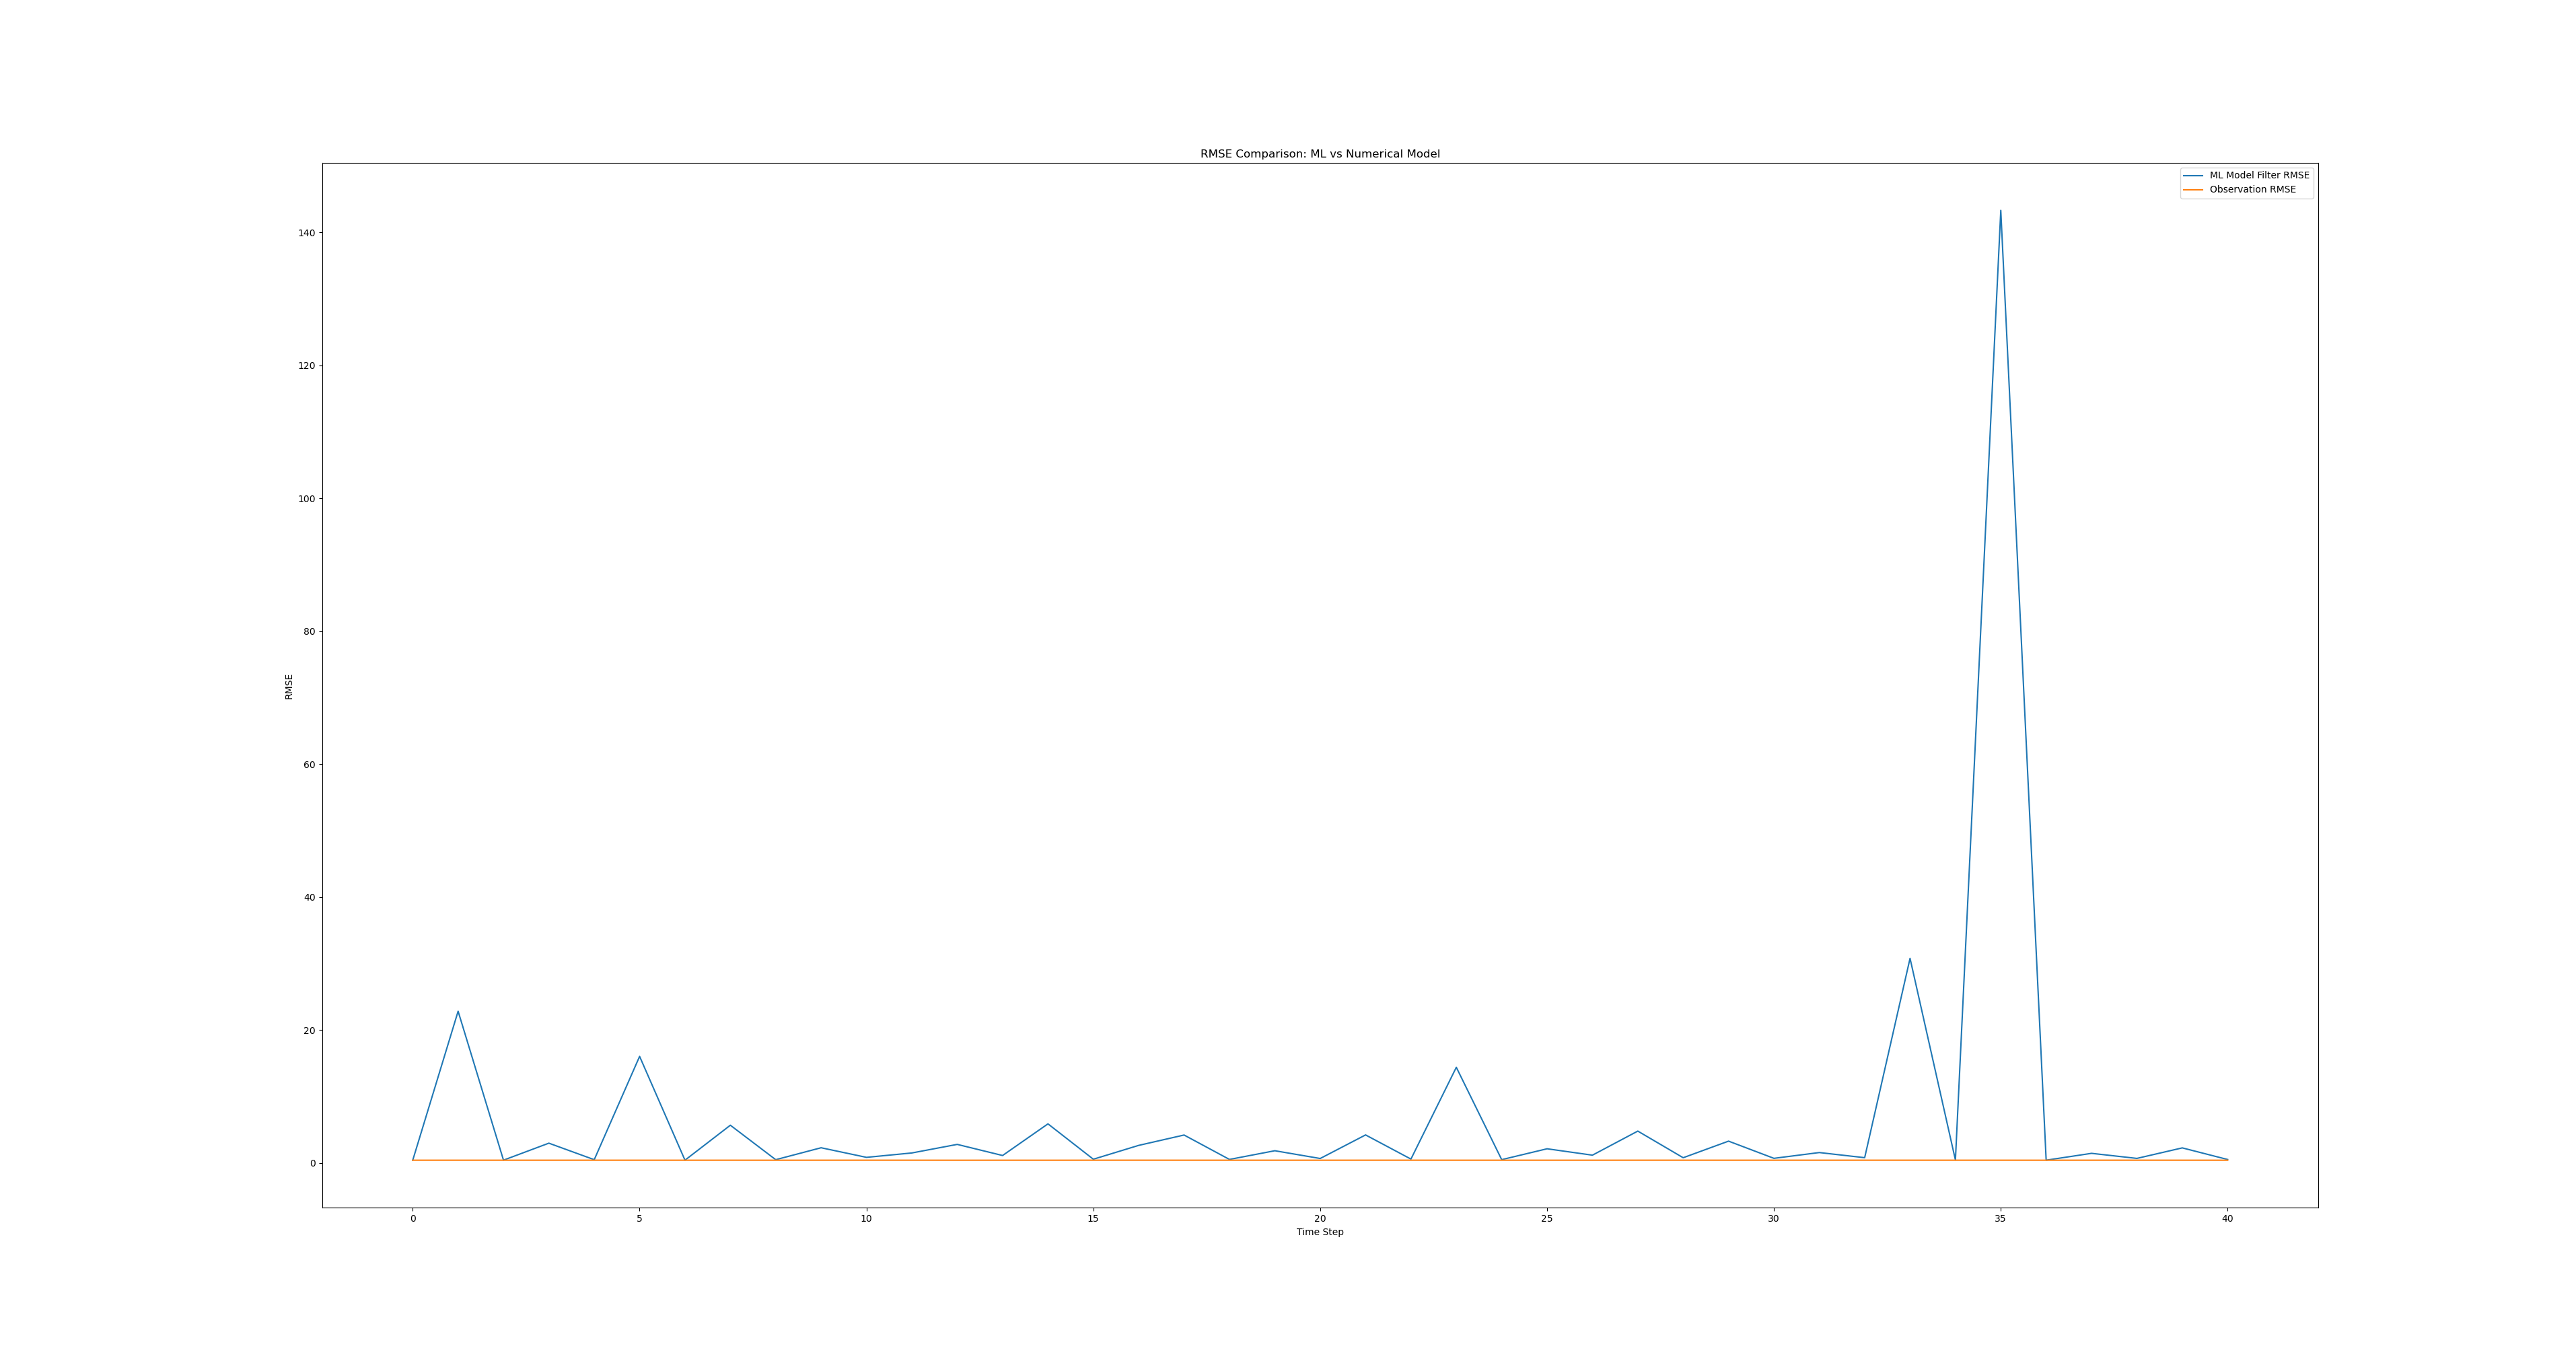
\includegraphics[width=\textwidth]{/mnt/c/workspace/study/Inverse Problem and Data Assimilation/pre/pic/n40_sz200_r2.png} % 替换为图片1的路径
        \caption{$r_{max}=2$}
    \end{minipage}%
    \hfill
    \begin{minipage}{0.32\textwidth}
        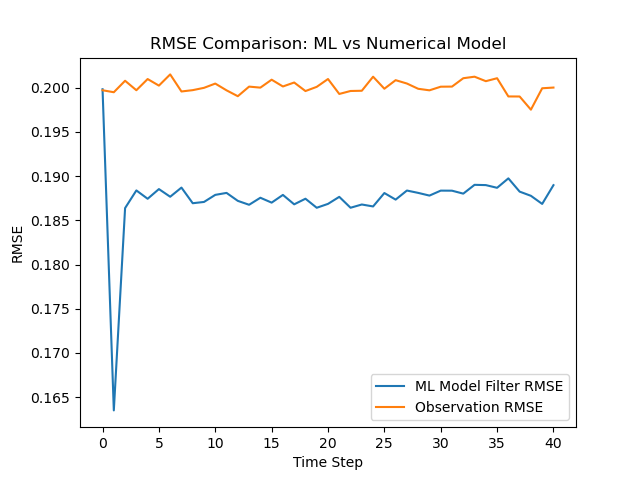
\includegraphics[width=\textwidth]{/mnt/c/workspace/study/Inverse Problem and Data Assimilation/pre/pic/n40_sz200_r3.png} % 替换为图片2的路径
        \caption{$r_{max}=3$}
    \end{minipage}%
    \hfill
    \begin{minipage}{0.32\textwidth}
        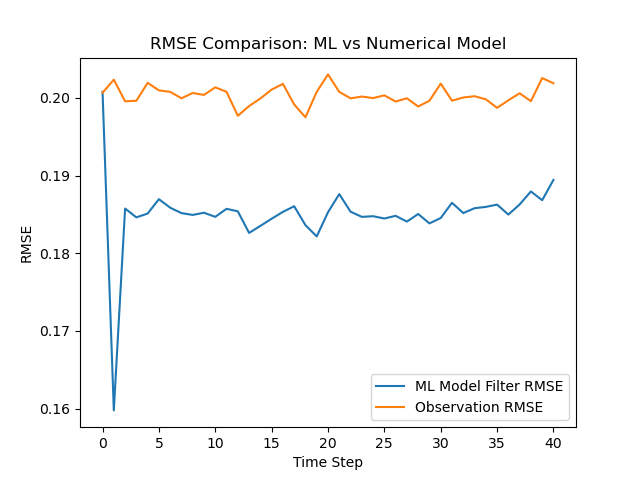
\includegraphics[width=\textwidth]{/mnt/c/workspace/study/Inverse Problem and Data Assimilation/pre/pic/n40_sz200_r4.png} % 替换为图片3的路径
        \caption{$r_{max}=4$}
    \end{minipage}
    My computer can't run for larger data, but the existing data and the trends mentioned in the original article are similar.
\end{figure}
\end{frame}
\section{Sequential processing of batches of observations}
\begin{frame}{Sequential processing of batches}
    \begin{columns}[c]
        % Left column for the image
        \column{0.5\textwidth}
        \centering
        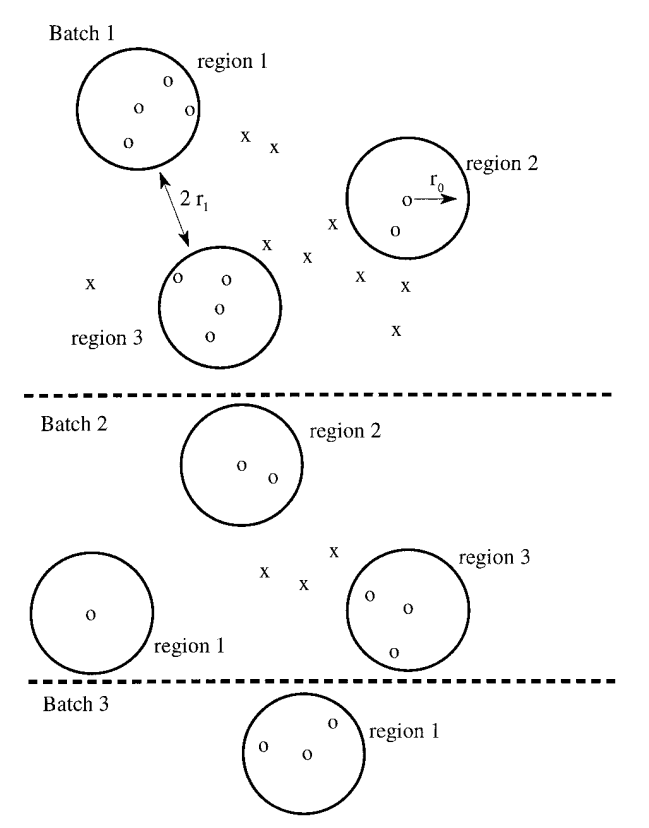
\includegraphics[width=\textwidth]{/mnt/c/workspace/study/Inverse Problem and Data Assimilation/pre/pic/batchs.png} % Replace with actual image file

        % Right column for the text
        \column{0.5\textwidth}
        In each batch, multiple regions that are far away from each other are selected for parallel assimilation, and the assimilation of a batch of observations is completed in multiple batches.

        It looks interesting, but I don’t know how to implement it yet. The observation method in the project is not consistent with that in the paper.
    \end{columns}
\end{frame}
\end{document}